\chapter{面向拜占庭容错的隐私保护梯度聚合技术}

\section{引言}
联邦学习(Federated Learning, FL)是目前主流的注重参与方数据隐私的分布式机器学习框架\cite{kairouz2019advances},它允许参与方不直接泄露本地数据的前提下,在FL服务提供商的协调下,完成联合全局模型的训练。
正是由于这种对原始数据的隐私保护,FL实现了一定程度上的数据可用不可见,也被许多企业在实际应用中落地。
比如谷歌使用FL打造了针对移动端用户的联合输入法预测系统\cite{hard2018federated},可以给用户提供更加精准的输入词推荐;微众银行基于FL部署了用户风险预测系统,更好的服务于对用户的风险评估服务。
粗略地说,FL主要有以下三个核心步骤:$(\rm \romannumeral1)$ FL服务提供商首先初始化随机的全局模型参数,然后分发给各个参与方;$(\rm \romannumeral2)$ 参与方收到全局模型参数后,将参数应用到本地,再使用本地数据集进行训练,更新本地参数,最后把更新后的参数(或梯度)上传给FL服务提供商;$(\rm \romannumeral3)$ 服务提供商接收到符合条件的参数数量之后,对参数进行聚合,生成新一轮的全局模型参数。
以上三个步骤一直被重复,直到联合训练的全局模型收敛。

尽管避免了对用户数据的直接泄露,相关文献\cite{kairouz2019advances, mothukuri2021survey, geiping2020inverting} 指出FL仍然面临着安全威胁,最典型的是针对用户梯度对用户数据进行反向推理的推理攻击 \cite{geiping2020inverting},以及可以操控参与方上传恶意参数更新的拜占庭攻击\cite{kairouz2019advances, mothukuri2021survey}。

(1)推理攻击:攻击的敌对方是不诚实的FL服务提供商,在接收到用户上传的参数之后,文献\cite{geiping2020inverting}指出FL提供商可以通过对参数进行余弦相似度的度量,再结合梯度的正负信息,反推出用户的隐私数据,这种攻击方式的存在也就意味着FL原来直接上传参数的方式,已经不能完全保证用户隐私了,需要使用进一步的隐私增强策略来保证用户隐私。%TODO Details

(2)拜占庭攻击:攻击的敌对方是可以操纵参与方的敌手 $\mathcal{A}$,在用户进行本地训练以及参数上传的阶段,敌手$\mathcal{A}$可以通过刻意构造所上传的参数,达到扰动或者控制全局模型收敛方向,或者侵犯其它参与方数据隐私的目的\cite{kairouz2019advances}。值得注意的是,文献\cite{blanchard2017machine}指出尽管只有一个参与方被敌手$\mathcal{A}$所控制,也能破坏整个FL流程的正常运行。

正是由于上述攻击行为对现有FL方案的隐私性和安全性提出的挑战,所以一个安全可信的FL系统,需要同时做到:$(\rm \romannumeral1)$进一步保护用户数据的隐私,避免隐私数据被服务提供商窃取;$(\rm \romannumeral2)$保证服务提供商聚合参数时的鲁棒性,剔除不良参数的影响。

要同时实现这两个目标,需要面对棘手的挑战。
一些前沿的提高FL拜占庭鲁棒性的方案\cite{blanchard2017machine, guerraoui2018hidden, yin2018byzantine}都假设聚合服务器是完全诚实的,也就是说,它不会从上传的用户模型参数中推断任何用户的隐私数据信息。
因此,这些工作都直接让用户上传原始的模型参数,然后在此之上构建拜占庭鲁棒的聚合方案。例如,Krum\cite{blanchard2017machine}基于用户模型参数在欧氏空间的相似性实现了一定程度上的拜占庭鲁棒性,当上传的用户参数为明文时,计算效率尚可接受。但是如果需要处理加密或者混淆过后的用户模型参数,计算可行性和计算效率将成为方案的瓶颈。
%然而,当参数被加密时,建立防御将是一个重大挑战,这意味着在密码文本域下识别拜占庭用户。

学者们提出了一系列工作\cite{liu2021privacy, dong2021flod, nguyen2022flame, hao2021efficient, so2020byzantine},致力于同时实现提升用户数据隐私以及聚合方案的拜占庭鲁棒性。
PEFL\cite{liu2021privacy} 使用同态加密(Homomorphic Encryption,HE)将用户本地梯度 $G_i$ 加密之后再上传到服务提供商,由两个半诚实非共谋的服务器完成鲁棒聚合,为了实现一些非线性操作,PEFL设计的四个安全计算协议都需要将 $G_i$ 使用随机数扰动之后,再进行解密操作。这里对于一个梯度 $G_i$ 的所有维度都使用相同的随机数进行扰动,这会泄露梯度数据的数据分布,存在隐私泄露的风险。FLOD \cite{dong2021flod} 和 SecureFL \cite{hao2021efficient} 方案都是基于FLTrust \cite{cao2020fltrust} 的根数据集(root dataset)思想,即服务提供商收集一小部分用户数据,用于判断和过滤恶意参数,显然这种方法会侵犯参与方的隐私。FLAME \cite{nguyen2022flame} 精心设计了拜占庭鲁棒聚合算法,并且结合ABY\cite{demmler2015aby} 以及隐私保护DBSCAN算法 \cite{bozdemir2021privacy} 实现了对用户梯度的隐私保护,但是其设计的鲁棒聚合算法涉及到安全两方计算(Secure 2-Party Computation,2PC)中开销较大的计算,其中包括梯度间余弦相似度的度量,以及共享份梯度的聚类操作。
表\ref{cmp}在隐私性、鲁棒性和效率上对已有工作和我们的工作进行了粗略的对比。

针对以上研究现状,本章提出了一个密文计算友好(即不涉及到开销较大的密文操作)的拜占庭鲁棒聚合方案,
并结合多方同态加密(Multiparty Homomorphic Encryption,MHE)实现了保证用户梯度隐私的同时,高效的在密文上剔除拜占庭用户的影响,具体来讲,我们的贡献如下:
\begin{compactenum}
	\item  我们提出了一个新颖的面向拜占庭容错的隐私保护联邦学习框架(Privacy-preserving and Byzantine-robust FL framework,PBFL),同时保证了用户数据的隐私和聚合后的全局梯度的隐私不被服务提供商窃取。同时,我们还避免了PEFL\cite{liu2021privacy}中存在的梯度数据分布泄露的问题。
	\item 我们设计了高效的、密文计算友好的拜占庭鲁棒聚合方案,它以用户参数到上一轮全局参数欧式距离的中值为基准,动态调节参与方每轮聚合的权重,使得每次聚合把恶意梯度的聚合权重降到可忽略的程度,充分发挥良性参数的作用。
	\item 我们对提出的方案在真实数据集上做了测试,实验表明我们可以有效的防御典型的拜占庭攻击,包括高斯攻击和标签转换攻击。除此之外,我们对方案进行了完备的安全性证明和收敛性证明,从理论上说明了方案可以在保护用户数据隐私的同时,实现对拜占庭节点的容错聚合。
\end{compactenum}

\begin{table}
	\centering
	\caption{Comparison with prior works on properties necessary for FL}
	\label{cmp}
	 \scalebox{0.90}{
		\renewcommand{\arraystretch}{1.2}
		\begin{tabular}{l|cccc}
			\toprule
			% \hline
			% \LEFTcircle \Circle \CIRCLE 
			\textbf{Proposed Schemes}               & \textbf{Approach}      & \textbf{Privacy}    &\textbf{Robustness} &\textbf{Efficiency}              \\
			\midrule
			PEFL \cite{liu2021privacy}                   & Custom Aggregation + HE & \CIRCLE\LEFTcircle     &\CIRCLE\LEFTcircle     &\CIRCLE\LEFTcircle                       \\
			FLAME \cite{nguyen2022flame}                   & Custom Aggregation + 2PC & \CIRCLE\CIRCLE     &\CIRCLE\LEFTcircle     &\LEFTcircle\Circle                       \\
			FLOD \cite{dong2021flod}                   & FLTrust \cite{cao2020fltrust} + 2PC & \CIRCLE\Circle     &\CIRCLE\CIRCLE     &\CIRCLE\LEFTcircle                       \\
			SecureFL \cite{hao2021efficient}                   & FLTrust \cite{cao2020fltrust} + 2PC & \CIRCLE\Circle     &\CIRCLE\CIRCLE     &\CIRCLE\LEFTcircle                       \\
			Our PBFL                   & Custom Crypto-friendly Aggregation + MHE & \CIRCLE\CIRCLE     &\CIRCLE\LEFTcircle     &\CIRCLE\CIRCLE                       \\
			\bottomrule
			% \hline
		\end{tabular}
		 }
\end{table}

本章的组织结构如下:在第\ref{bg}节和第\ref{ps}节我们分别介绍了本章方案涉及到的一些预备知识和方案要解决的问题描述;
然们我们在第\ref{friendly-alg}节和第\ref{PBFL}节对提出的面向拜占庭容错的隐私保护梯度聚合方案进行了细致的描述;接下来在第\ref{ana}节对方案就行了安全性分析、收敛性分析以及效率分析;在第\ref{con}节对本方案进行了实验评估;最后在第\ref{con}节对本方案进行了总结。

\section{预备知识}\label{bg}

\subsection{联邦学习}
联邦学习(Federated Learning,FL)是目前前言的分布式机器学习方案,它可以让许多参与方(比如终端用户)在中央服务器的调度下,完成联合的机器学习或者深度学习训练,同时保证参与方数据留存在本地。在FL中,中央服务器负责整个训练任务的初始化、以及训练过程中用户参数的聚合以及分发;而参与方负责使用本地数据优化收到的全局模型参数,然后将更新之后的参数上传给中央服务器。

本方案的训练任务集中在经典的有监督学习任务,即图像分类的学习任务。
具体来说,参与方 $P_i$ 持有本地隐私数据集 $D_i=\{(x_j, y_j);j=1,2,...,T\}$,其中$x_j\in\mathbb{R}^v$表示一个$v$维度的图像向量,而 $y_i$ 是该图像的真实标签。
在训练轮次 $t$ 的开端,服务器会把全局参数 $W_g$ 分发给参与到训练的参与方,每个参与方 $P_i$ 将收到的全局参数 $W_g$ 应用到本地模型,然后使用本地数据集 $D_i$ 本地计算loss函数,计算方式如下:
\begin{equation}
	\mathcal{L}_f(D_i, W_g) \leftarrow\frac{1}{|D_i|}\sum\limits_{(x_j,y_j)\in D_i}\mathcal{L}_f(x_j,y_j,W_g),
\end{equation}
其中$\mathcal{L}_f(x_j,y_j,W_g)$是计算模型输出以及图像真实标签之间差异的loss值。
FL的目标是通过最小化全局loss函数的方式,获得最优的全局模型参数。
在本方案中,我们利用随机梯度下降算法(stochastic gradient descent,SGD)来更新本地模型参数。
即每个参与方对于$D_i$中的小批量数据$D_i^k \in D_i$,执行如下计算:
\begin{equation}
	W^{k+1}\leftarrow W^{k}-\eta\nabla\mathcal{L}_f(D_i^k,W^k)
\end{equation}
其中$k$代表本地训练周期。在本地参数更新完成之后,参与方$P_i$会获取到本轮更新的全局参数 $W_i^t$,然后将其发送给中央聚合服务器,等待服务器完成线性聚合:
\begin{equation}
	W_g^{t}\leftarrow\sum_{i=1}^{N}\frac{1}{N}W_i^{t},
\end{equation}
其中 $N$ 表示参与方的数量。参与方和服务器重复上述过程,直到全局模型收敛。

\subsection{非目标性的拜占庭攻击}
在我们的拜占庭威胁模型中,敌手 $\mathcal{A}$ 可以控制一部分FL的参与方,这些参与方也被称为拜占庭用户。
这些拜占庭用户可以不向服务器发送更新的模型参数,而是发送任意的或精心构建的参数,来影响全局模型的准确率。
本方案考虑了两种典型的非目标性的拜占庭攻击,即模型毒化攻击(Model poisoning attack)和数据毒化攻击(Data poisoning attack),具体描述如下:
\begin{compactitem}
	\item \textbf{模型毒化攻击:}这种攻击行为发生在本地用户的训练阶段,敌手 $\mathcal{A}$ 可以直接更改用户需要上传的模型参数,比如说可以胁迫参与方替换上传的参数为随机选取的高斯噪声,也被称为高斯攻击(Gaussian attack,GA)\cite{blanchard2017machine, dong2021flod},GA可以导致全局模型的大幅波动,从而严重影响全局模型的收敛。
	\item  \textbf{数据毒化攻击:}这种攻击通常发生在参与方数据的收集阶段,敌手$\mathcal{A}$ 可以修改用户收集到的本地数据,将数据的真实标签修改为错误的虚拟标签。比如说对于一张手写数字图片,其真实内容和标签都是5,而敌手$\mathcal{A}$可以保持图像数据特征不变,将标签改为9,从而影响全局模型的准确率,这种具体的攻击也被称为标签转换攻击(Label-flipping attack,LFA)\cite{kairouz2019advances, dong2021flod, liu2021privacy}。这种攻击可以破坏全局模型收敛的方向,从而大幅降低全局模型的准确率。
\end{compactitem}

\subsection{多方同态加密}
我们的隐私保护计算模块基于的是一种全同态加密(Cheon-Kim-Kim-Song,CKKS\cite{cheon2017homomorphic})的修订方案,即多方同态加密(Multiparty Homomorphic Encryption,MHE)。
在MHE中,可以由多个参与方本地持有私钥,然后在不泄露本地私钥的前提下,协同生成一份公钥。
而密文的解密操作则需要所有持有私钥的参与方一起完成。
我们选择使用MHE构建本方案的理由如下:
$(\rm \romannumeral1)$ 该方案原生支持浮点数计算,这非常契合网络模型参数中都为浮点数的场景。
$(\rm \romannumeral2)$ 该方案基于环上的困难问题(ring learning with errors,RLWE)搭建,可以让我们的方案实现抗量子攻击(post-quantum attacks)。
$(\rm \romannumeral3)$ 其密文上的计算可以做到灵活且非交互。
$(\rm \romannumeral4)$ 其支持安全的合作公钥切换操作,即在不解密一个密文的前提下,完成对密文的重加密(即用给定的另一份公钥加密),接下来我们对MHE方案进行简单介绍。

在MHE中,分圆多项式环的次数表示为 $\mathcal{N}$(取值为2的整数次方),决定了MHE的明文和密文空间分别为$R_{Q_{L}}=\mathbb{Z}_{Q_{L}}[X]/(X^{\mathcal{N}}+1)$和$Q_{L}=\prod_{0}^{L}q_i$,其中 $q_i$ 表示特定的素数,$Q_L$ 是初始等级为 $L$ 的密文模数。
我们在图\ref{f1}中简单介绍了我们使用到的MHE相关函数。在图中,我们使用$\llbracket c\rrbracket_{pk}=(c_0,c_1)\in R^2_{Q_{L}}$ 和 $\overline{p}\in R_{Q_{L}}$ 分别表示MHE公钥加密后的密文和编码之后的明文,其它的符号描述可以参考\ref{tab:symbol}。
%我们分别使用 $L_c$, $S_c$, $L$, $S$ 表示
%TODO 这里的MHE概念加一点自己的理解
%TODO 描述改成脚注
%SUb
%POWER -> Mult -> rel
%InnerSum -> rotL/R + add
%Add
%MultByConst 
% 考虑用圈圈起来的符号,表示密文运算,
%  加法减法、求和简单来
在描述图\ref{f1}中,以$‘\textbf{D}’$开头的函数都是分布式的,需要由所有私钥持有方一起完成,而其它的函数在任意一方本地计算即可。

\begin{table}[htbp]
	\centering
	\begin{minipage}[t]{0.6\linewidth}
		\caption{MHE相关函数描述的符号标注}
		\label{tab:symbol}
		\begin{tabular*}{\linewidth}{lp{10cm}}
			\toprule[1.5pt]
			{\hei 符号} & {\hei 描述}\\
			\midrule[1pt]
			$L_c$ & 密文$\llbracket c\rrbracket_{pk}$当前的密文等级 \\ 
			$S_c$ & 密文$\llbracket c\rrbracket_{pk}$当前的缩放量\footnote{缩放量是指密文解密后的明文和真实表示的明文之间的固定倍数关系} \\
			$L$ & 密文的初始化等级\\
			$S$ & 密文的初始化缩放量\\
			\bottomrule[1.5pt]
		\end{tabular*}
	\end{minipage}
\end{table}

\begin{figure}[!htb]
	\begin{framed}
		\noindent \textbf{SecKeyGen($1^\lambda$):} Returns a set of secret keys ${sk_i}$,\\
		i.e., $sk_i$ for user $P_i$ with the given security parameter $\lambda$.\\
		\noindent \textbf{DKeyGen(${sk_i}$):} Returns a collective public key $pk$.\\
		\noindent \textbf{DRelinKeyGen(${sk_i}$):} Returns a collective public key $rlk$.\\
		\noindent \textbf{DRotKeyGen(${sk_i}$):} Returns a collective public key $rtk$.\\
		\noindent \textbf{Encode($msg$):} Returns a plaintext $\overline{p}\in R_{Q_{L}}$ with scale $S$, encoding $msg$, a complex vector.\\
		\noindent \textbf{Decode($\overline{p}$):} With $\overline{p}\in R_{Q_{L}}$ and scale $S_{\overline{p}}$, returns the decoding complex vector of $\overline{p}$.\\
		\noindent \textbf{DDecrypt($\llbracket c\rrbracket_{pk}, {sk_i}$):} With $\llbracket c\rrbracket_{pk}\in R^2_{Q_{L}}$ and scale $S_c$, returns the plaintext $p\in R_{Q_{L}}$ with scale $S_c$.\\
		\noindent \textbf{Enc($pk, \overline{p}$):} Returns ciphertext $\llbracket c\rrbracket_{pk}\in R_{Q_{L}}$ \\
		with scale $S$.\\
		\noindent \textbf{Add($\llbracket c\rrbracket_{pk}, \llbracket c^{\prime}\rrbracket_{pk}$):} Returns $(\llbracket c+c^{\prime}\rrbracket_{pk})$ \\
		at level min($L_c, L_{c^{\prime}}$) and scale max($S_c, S_{c^{\prime}}$).\\
		\noindent \textbf{Sub($\llbracket c\rrbracket_{pk}, \llbracket c^{\prime}\rrbracket_{pk}$):} Returns $(\llbracket c-c^{\prime}\rrbracket_{pk})$ \\
		at level min($L_c, L_{c^{\prime}}$) and scale max($S_c, S_{c^{\prime}}$).\\
		\noindent $\textbf{Mul}_{ct}$$(\llbracket c\rrbracket_{pk}, \llbracket c^{\prime}\rrbracket_{pk})$: Returns $\llbracket cc^{\prime}\rrbracket_{pk}$ at level min($L_c, l_{c^{\prime}}$), scale ($S_c\times S_{c^{\prime}}$).\\
		\noindent \textbf{Power}$(\llbracket c\rrbracket_{pk}, n)$: Returns $\llbracket c^{n}\rrbracket_{pk}$ at level $(S_c-\log{n})$\\
		\noindent \textbf{RotL/R}($\llbracket c\rrbracket_{pk}, k$): Homomorphically rotates $\llbracket c\rrbracket_{pk}$ to the left/right by $k$ times.\\
		\noindent \textbf{DPubKeySwitch}$(\llbracket c\rrbracket_{pk}, pk^{\prime},{sk_i})$: Returns $\llbracket c\rrbracket_{pk^{\prime}}$\\without decryption.\\
		\noindent $\textbf{MulByConst}(\llbracket c\rrbracket_{pk}, const)$: Returns $\llbracket c\times const\rrbracket_{pk}$ with scale depends on $S_c$ and $const$, at level $L_c$.\\
		% \noindent $\textbf{InnerSum}(\llbracket c\rrbracket_{pk}, batchSize, n)$: Returns $\llbracket c^{\prime}\rrbracket_{pk}$, the sum of $n$ sub-vector with $batchSize$ dimensions in vector hidden in $\llbracket c\rrbracket_{pk}$.
		\noindent $\textbf{InnerSum}(\llbracket c\rrbracket_{pk})$: Returns $\llbracket c^{\prime}\rrbracket_{pk}$, the inner sum of vector hidden in $\llbracket c\rrbracket_{pk}$.
		% \textbf{Our expansion, two sub-steps in DDecrypt:}\\
		% \textbf{1.PartDec}($\llbracket c\rrbracket_{pk},sk_i$): Returns a part of the decryption information $h_i$.\\
		% \textbf{2.AggDec}$(\llbracket c\rrbracket_{pk},\{h_i\})$: Returns the plaintext $p\in R_{Q_{L}}$ with scale $S_c$.
	\end{framed}
	\caption{Frequently used cryptographic operations in MHE}
	\label{f1}
\end{figure}


\section{问题描述}\label{ps}

\subsection{系统模型}
我们的系统模型图如图\ref{syspnd},其中主要有四个实体,具体描述如下:
\begin{compactitem}
	\item \textit{聚合服务器(Aggregation Server,AS):}AS为所有的FL参与方提供协同训练的聚合服务。在每个FL轮次中,AS收集用户上传的加密模型参数,然后聚合生成全局模型参数后分发给用户。
	\item \textit{密码服务提供商(Crypto Service Provider,CSP):}CSP负责辅助AS完成对用户上传的加密模型参数的聚合,即CSP持有一份私钥,在不侵犯用户参数隐私的前提下,利用私钥计算AS需要的中间信息。
	\item \textit{数据拥有者(Data Owners,Parties in FL):}FL中需要联合训练的参与方,在本地持有隐私数据。本方案假定数据持有者可能被敌对方挟持,做出恶意行为扰乱FL系统。
	\item \textit{密钥生成助手(Key Generation Assistant,KGA):}KGA协助所有参与方和AS生成用户侧的公私钥对,且保证参与方收到的私钥是同一份。为了避免KGA的独立解密行为,我们让其和AS分别持有一份私钥,并且假设KGA是半诚实(semi-honest)实体且不和AS发生共谋行为,KGA在完成密钥生成之后,将持有的私钥安全的分发给所有参与方。
\end{compactitem}

\begin{figure}[htbp]
	\begin{center}
		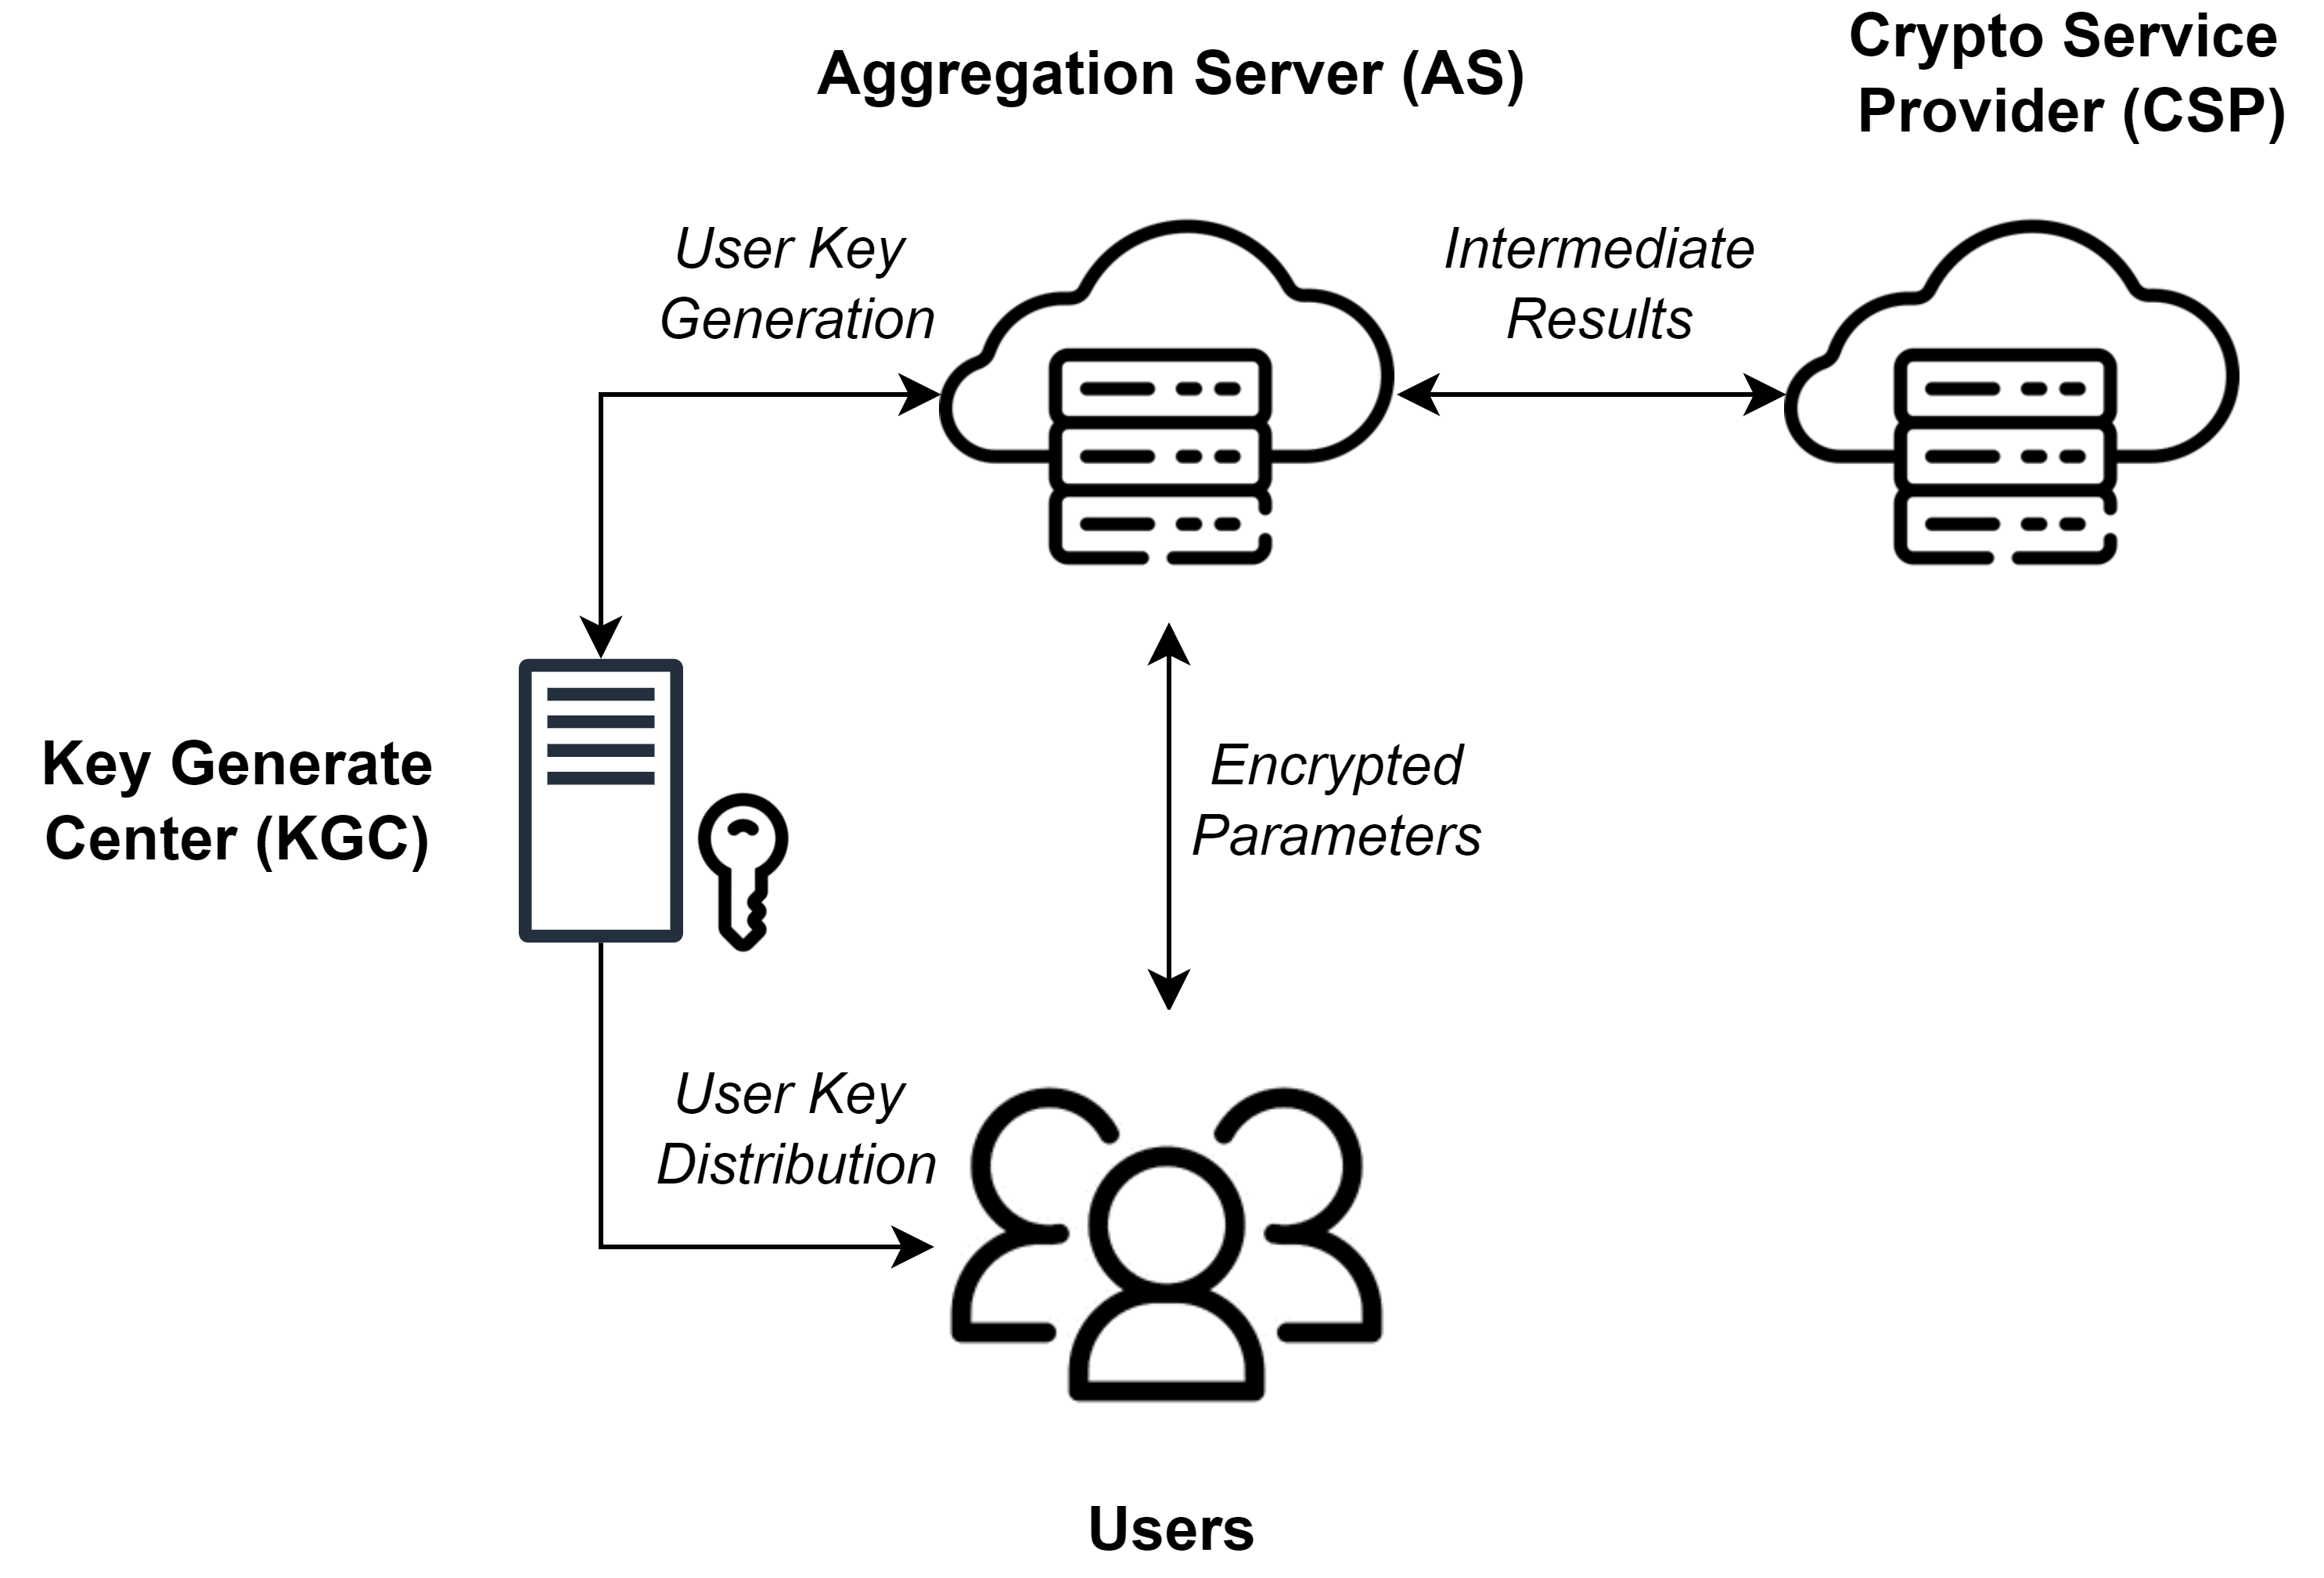
\includegraphics[scale=0.077]{img/sys-v3.drawio.png}
		\caption{系统模型图}
		\label{syspnd}
	\end{center}
\end{figure}

\subsection{威胁模型}
本方案致力于同时解决由半诚实聚合服务器造成的隐私威胁和由拜占庭用户造成的安全威胁。我们假设FL中的参与方的本地数据是独立同分布的(independent identically distributed,IID)。
拜占庭用户可以向AS发送任意的模型参数,从而影响全局模型的训练。
同时本方案与类似工作\cite{so2020byzantine, yin2018byzantine, liu2021privacy}持有同样的假设,我们假定拜占庭用户的上限不超过所有用户的一半,即$|M|\leq\frac{|T|-1}{2}$,其中$|M|$ 和 $|T|$ 分别表示恶意用户的数量和所有用户的数量,这个假设是本方案收敛性证明的前提。
除此之外,我们假设AS、CSP和KGA是半诚实实体,这意味着它们将严格执行本方案设计的安全协议,并且尝试从中推断出用户的隐私信息。
最后,我们假设方案中涉及到的四个实体AS、CSP、KGA和Users,都不会和其它任意一方发生共谋行为。

\subsection{设计目标}
基于以上提到的系统模型和威胁模型,本方案需要达到的目标如下:
\begin{compactitem}
	\item \textbf{保护模型参数隐私:}实现对用户上传的本地参数和聚合后的全局参数的隐私保护,保证模型参数对AS和CSP而言,可用而不可见。
	\item \textbf{实现拜占庭容错:}对于可能出现的最多半数的拜占庭用户,本方案将实现在密文上的拜占庭用户过滤,保证全局模型的准确率。
	\item \textbf{提升全局模型准确率:}对比现有的其它方案,实现在相同恶意环境下的全局模型准确率的提升。
\end{compactitem}

\section{拜占庭鲁棒参数聚合算法}\label{friendly-alg}
本节我们详细描述设计的密文计算友好的拜占庭容错梯度聚合协议。本方案涉及到的符号在表\ref{sym}中就行了具体的描述。

为了涉及密文计算友好的拜占庭容错参数聚合算法,我们提出了高效的距离计算基准选择以及有效的聚合权重赋予策略,详细描述如下:
\begin{compactitem}
	\item \textbf{高效的距离计算基准选择:}我们对用户本地参数进行评估时,需要一个基准来判断用户参数的质量,即我们使用计算参与方参数到基准参数的距离,决定参数的聚合权重(将权重赋予良性梯度)。我们观察到,参与方的本地模型参数和上一轮的全局参数的距离,反映了用户本轮次更新的幅度大小,因此我们选择使用\textbf{上一轮的全局模型},作为距离计算的基准。这很好的提升了本方案的密文友好性和计算复杂度,对比PEFL\cite{liu2021privacy}我们不需要进行复杂的参数基准计算(增加密文计算开销),即将基准的计算从复杂度$ O(N) $降低到了常数复杂度$ O(1) $,其中$N$表示参与方的数量。
	\item \textbf{基于中值的权重赋予策略:}针对我们选择的计算基准(上一轮的全局模型),拜占庭用户可以从两方面进行攻击,$(\rm \romannumeral1)$进行幅度很小的更新或不更新,以此扰乱全局模型的收敛;$(\rm \romannumeral2)$进行幅度很大的更新,破坏全局模型更新的方向。因此,我们将到基准的距离较小和较大的用户更新视为恶意更新,然后赋予较小甚至可忽略的聚合权重。而距离值位于中间的参与方,我们将其视为良性参与方,赋予较高的聚合权重,我们对算法的细节在算法\ref{a0}中进行了详细的描述。
\end{compactitem}
\begin{table}
	\centering
	\caption{符号表}
	\label{sym}
	\scalebox{0.95}{
		\renewcommand{\arraystretch}{1.2}
		\begin{tabular}{cl}
			\hline
			\hline
			\textbf{符号}               & \textbf{描述}                      \\ 
			\hline
			$\lambda$                      & 安全参数                        \\ 
			$pk_x$                         & 实体$x$的公钥                              \\ 
			$sk_x^y$                       & \makecell[l]{实体$y$持有的对应于公钥$ pk_x $的私钥} \\ 
			$D$                            & 用户本地数据                             \\ 
			$x$                            & 数据样本特征                   \\ 
			$y$                            & 数据样本标签                              \\ 
			$W_g$                            & 全局模型参数                            \\ 
			$W_i$                            & 用户$P_i$本地模型参数                             \\ 
			$G$                            & 模型梯度                           \\ 
			$\eta$                         & 模型训练学习率                          \\ 
			$N$                            & FL中参与方数量                 \\ 
			$\llbracket W \rrbracket_{pk}$ & 使用公钥$pk$加密的密文 \\ 
			$d$                            & 欧式距离           \\ 
			$f_s(P_x, t)$                  & \makecell[l]{在轮次t,表示计算出参与方$ P_x $聚合权重的抽象函数} \\
			$\gamma_i$                       & 参与方$P_i$的聚合权重       \\
			\hline
			\hline
		\end{tabular}
	}
\end{table}

\begin{algorithm}[htbp]
	\caption{密文计算友好的拜占庭鲁棒FL聚合协议}
	\label{a0}
	\begin{algorithmic}[1]
		\REQUIRE 在轮次$t$,参与方本地模型参数 $\{W_1^t, W_2^t, ..., W_N^t\}$,其中$N$表示参与方数量,$W_g^{t-1}$ 表示上一轮的全局模型参数。
		\ENSURE 轮次$t$ 的全局模型参数 $W_g^t$。 
		\FOR{$i \in [1...N]$ 计算用户参数到基准的欧式距离平方}
		\STATE ${d}_i = \Vert W_i^t - W_g^{t-1} \Vert ^2$
		\ENDFOR
		\STATE 获取距离向量 ${d}$的中值:\\${d}_{mid} = median(\{{d}_{1}, {d}_{2},..., {d}_{n}\})$
		\FOR{$i\in[1...N]$ 计算到 $d_{mid}$ 的距离}
		\STATE $d^{\prime}_{i}=\left|d_i-d_{mid}\right|$
		% \STATE $d^{\prime}_{sum}=d^{\prime}_{sum}+d^{\prime}_{i}$
		\ENDFOR
		% \STATE Obtains the sum of the individual values in vector $d$ as $d_{sum}$
		\FOR{$i\in[1...N]$} %calculates the relative distance to $d_{mid}$}
	\STATE $scores_i=\dfrac{\sum_{j=1}^{N} (d^{\prime}_{j} + 1)}{d^{\prime}_i + 1}$ \COMMENT{距离$ d_{mid} $越近,聚合权重越高}
	\ENDFOR
	\FOR{$i\in [1...N]$ 缩放 $scores_i$ 到 0-1}
	\STATE $\gamma_i=\dfrac{scores_i}{\sum_{j=1}^{N} scores_j}$
	\ENDFOR
	\STATE 使用缩放后的权重线性聚合参数:\\
	$W_g^{t} =\sum_{i=1}^{N}\gamma_i * W_i^{t}$
\end{algorithmic}
\end{algorithm}

\section{隐私保护的拜占庭鲁棒梯度聚合方案}\label{PBFL}
本节详细描述了本方案如何赋予我们设计的拜占庭鲁棒聚合算法完全的模型参数隐私保护能力。
粗略的说,首先用户将使用HE加密后的本地模型更新,上传到AS,然后AS在CSP的协助下,
在密文上确定每份本地更新的聚合权重,聚合完成后再完成全局参数的安全分发。主要有如下四个阶段:系统初始化、本地训练、参数的隐私安全聚合以及参数的安全分发。

\subsection{系统初始化}
本阶段需要完成两对非对称密钥的生成与分发,首先AS和CSP协同生成服务端侧密钥(下标以$ s $注明),其协同调用四个MHE安全协议SecKeyGen($\cdot$), DKeyGen($\cdot$), DRelinKeyGen($\cdot$), 和 DRotKeyGen($\cdot$),协同生成一份密钥集合$$ (pk_s, rlk_s, rtk_s, sk_{s}^{AS}, sk_{s}^{CSP}),$$其中私钥$ sk_{s}^{AS} $由AS持有,私钥$ sk_{s}^{CSP} $由CSP持有,其余密钥公开,$ pk_s $用于明文的加密,$ rlk_s $用于密文乘法后的重线性化,$ rtk_s $y用于计算内部元素和时的元素移动。

然后KGA和AS之间协同生成用户侧密钥(下标以$ u $注明),通过执行SecKeyGen($\cdot$) 和 DKeyGen($\cdot$)协议,生成$(pk_u, sk_{u}^{AS}, sk_{u}^{U})$,其中私钥$ sk_{u}^{AS} $由AS持有,$ sk_{u}^{U} $ 由KGA持有,然后安全分配给所有用户(所有用户持有相同私钥)。在这个过程中,KGA充当一个中介,使得所有用户和AS协商得到一份公私钥集合,为了保证KGA不直接持有用户侧私钥,对用户隐私造成威胁,我们选择使AS和KGA同时持有私钥,同时假设AS和KGA之间没有共谋行为。

服务器侧公钥用于加密用户上传的本地参数,将私钥分布于AS和CSP之间为了保证AS不能直接解密用户上传的加密参数;而用户侧的公钥用于加密聚合后的参数,将私钥分布与AS和所有用户之间,为了保证AS或者CSP不能直接解密聚合后的参数。以此我们实现了对本地参数以及聚合后全局参数的隐私保护,具体的私钥分配示意图如图\ref{keypng}所示。

\begin{figure}[htbp]
	\begin{center}
		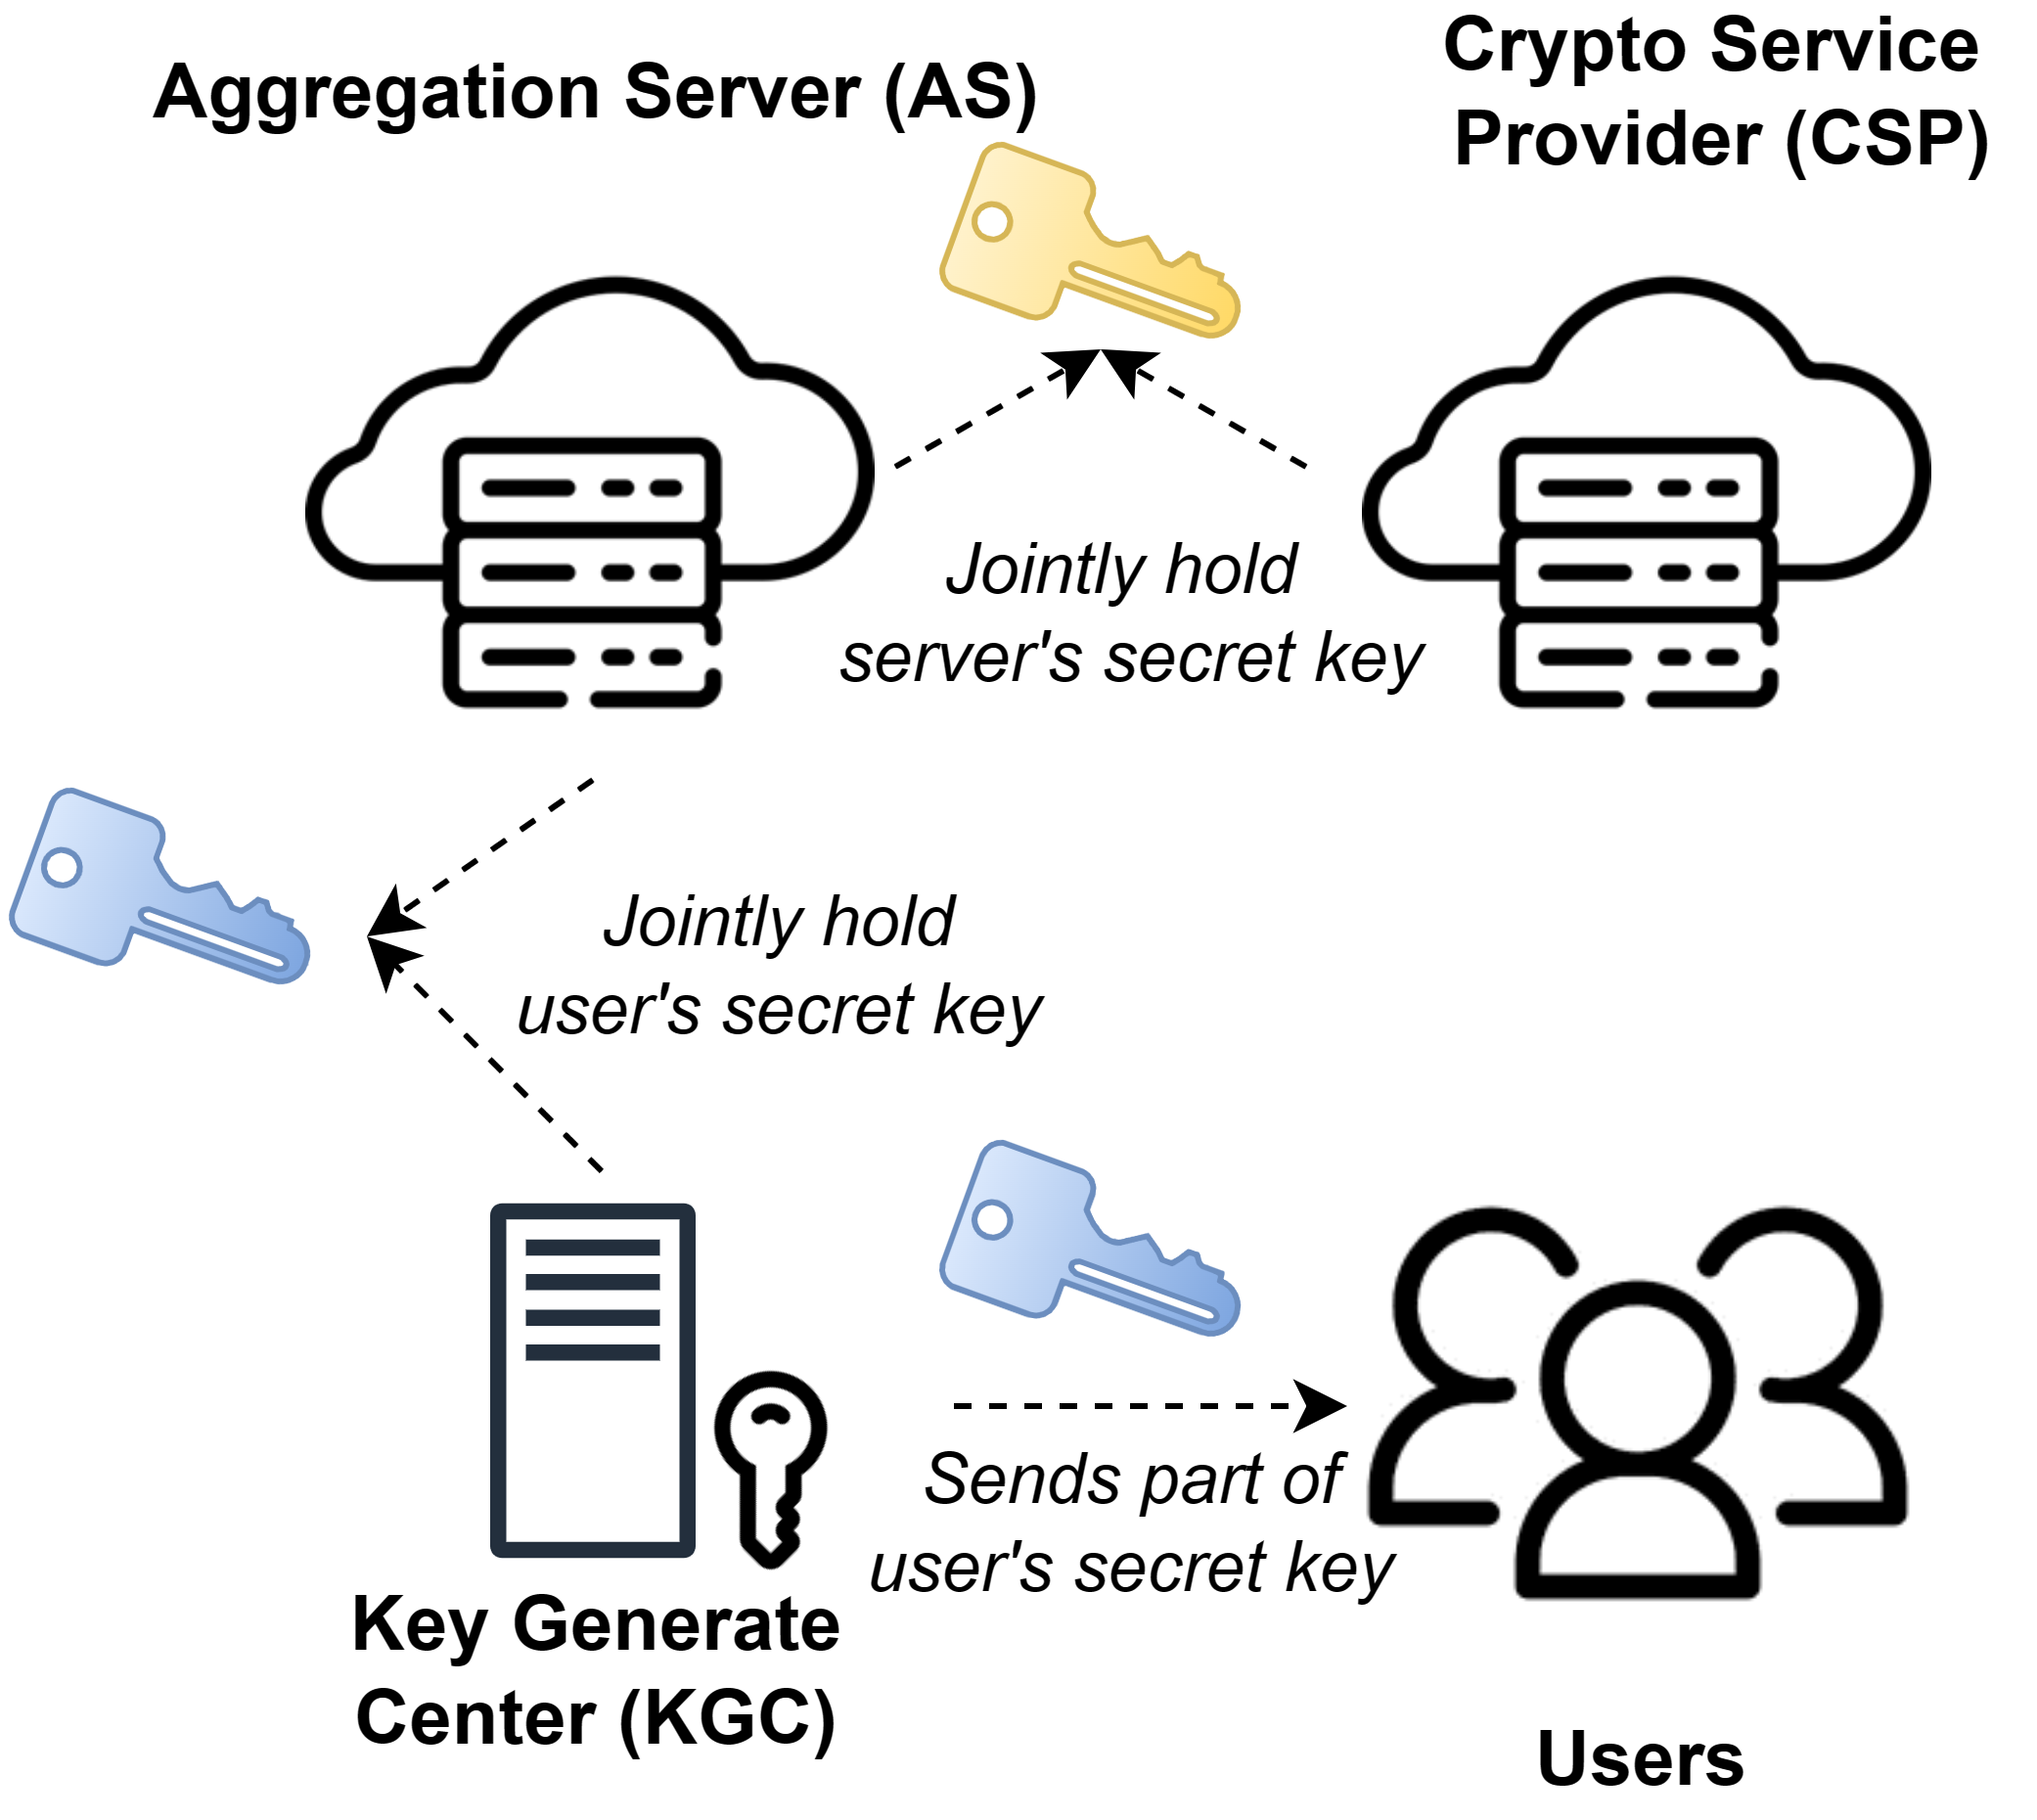
\includegraphics[scale=0.077]{img/key-v1.drawio.png}
		\caption{私钥分布示意图}
		\label{keypng}
	\end{center}
\end{figure}

从密钥分配方案可知,本方案的私钥皆由两方持有,于是我们对MHE进行了两方安全计算协议的设计,其中包括安全的两方协同解密算法(Secure 2-party cooperative decryption,\textbf{Sec2Dec})和安全的两方协同公钥切换算法(Secure 2-party cooperative public key switch,\textbf{Sec2KeyS})。
\textbf{Sec2Dec}和\textbf{Sec2KeyS}以如下两个MHE分布式函数为基础:
\begin{compactitem}
	\item \textbf{DDecrpted($\cdot$)}:其联合所有私钥持有方解密密文 $\ctx[pk]{c}$。以两方$P_1, P_2$ 分别持有私钥 $sk_1, sk_2$ 为例,为了解密密文 $\ctx[pk]{c}$,$P_1$ 和 $P_2$ 在本地分别利用私钥计算本地部分解密结果 $ h_1 $ 和 $ h_2 $,然后由一方收集所有本地解密结果,聚合得到密文的解密结果。这个分布式解密过程,可以做到对聚合方之外的另一方保密。为了方便描述,我们将这两个子过程分别描述为部分解密 PartDec$(\cdot)$ 和解密结果聚合 AggDec$(\cdot)$。
	\item  \textbf{DPubKeySwitch($ \cdot $)}:其联合所有私钥持有方在不解密密文的前提下,对密文进行加密公钥的切换。同样以两方$P_1, P_2$ 分别持有私钥 $sk_1, sk_2$ 为例,为了将密文$ \ctx[pk]{c} $切换为由公钥 $ \ctx[pk^{\prime}]{c} $加密,$ P_1,P_2 $在本地利用私钥进行部分的公钥切换运算,然后再交由一方聚合所有的本地运算结果。整个分布式公钥切换的过程,不会泄露原始明文。为了简化描述,我们将两个子步骤描述为本地计算的部分公钥切换PartSwitch($\cdot$) 和切换结果聚合AggSwitch($\cdot$)。
\end{compactitem}
具体的子步骤描述如图\ref{f2}所示。
\begin{figure}
	\begin{framed}
		\textbf{DDecrypt($\cdot$)}子步骤:\\
		\indent\textbf{1.PartDec}($\llbracket c\rrbracket_{pk},sk_i$): 返回本地部分解密信息 $h_i$。\\
		\indent\textbf{2.AggDec}$(\llbracket c\rrbracket_{pk},\{h_i\})$: 返回明文 $c\in R_{Q_{L}}$。\\
		
		\textbf{DPubKeySwitch($ \cdot $)}子步骤:\\
		\indent\textbf{1.PartSwitch}($\llbracket c\rrbracket_{pk},{sk_i},pk^{\prime}$): 返回本地部分公钥切换信息 $s_i$.\\
		\indent\textbf{2.AggSwitch}$(\{s_p\})$: 返回以新公钥$ pk^{\prime} $加密的密文 $\llbracket c^{\prime}\rrbracket_{pk^{\prime}} \in R^2_{Q_{L}}$。
	\end{framed}
	\caption{MHE分布式函数步骤划分}
	\label{f2}
\end{figure}

\textbf{Sec2Dec}是MHE中的分布式协同解密算法\textbf{DDecrypt($\cdot$)}在两方场景下的定制化。具体来说,我们两方持有密文,需要另一方协同解密但又不向另一方泄露明文的场景,进行了设计。
假设私钥持有方$p_1,p_2$\footnote{$p_1,p_2$可以是方案实体中的任意两方,比如AS和CSP}分别持有私钥$sk^1, sk^2$,其对应公钥为$ pk $,$ p_1 $和$p_2$持有密文$\ctx[pk]{c}$,需要在对$p_2$保密的前提下,解密$\ctx[pk]{c}$,算法的细节描述如算法\ref{a-1}所示。
\begin{algorithm}[htbp]
	\caption{安全两方协同解密算法\\ \textbf{Sec2Dec}($\{sk^1, sk^2\}, \llbracket c\rrbracket_{pk}$) $\rightarrow c$}
	\label{a-1}
	\begin{algorithmic}[1]
		\REQUIRE 对于MHE密钥集合$(\{sk^1, sk^2\}, pk)$,参与方 $p_1$ 和 $p_2$ 分别持有 $sk^1$ 和 $sk^2$;$p_1, p_2$ 持有密文 $\llbracket c\rrbracket_{pk}$.
		\ENSURE 参与方 $p_1$ 获取明文 $c$, 且 $c$ 对$ p_2 $保密。
%		\IF{参与方 $p_2$ 不持有 $\llbracket c\rrbracket_{pk}$}
%		\STATE $p_1$ 发送 $\llbracket c\rrbracket_{pk}$ 给 $p_2$.
%		\ENDIF
		\FOR{$x \in \{1, 2\}$}
		\STATE 参与方 $p_x$ 计算部分解密信息如下:\\ $\llbracket c_x\rrbracket_{pk} \leftarrow \textbf{PartDec}(\llbracket c\rrbracket_{pk}, sk^x)$. 
		\ENDFOR
		\STATE 参与方 $p_2$ 发送 $\llbracket c_2\rrbracket_{pk}$ 到 $p_1$。
		\STATE 参与方 $p_1$ 聚合部分解密信息如下:\\ $c \leftarrow \textbf{AggDec}(\llbracket c\rrbracket_{pk}, \{\llbracket c_1\rrbracket_{pk}, \llbracket c_2\rrbracket_{pk}\})$
		\RETURN $p_1$ 获取明文 $ c $.
	\end{algorithmic}
\end{algorithm}

\textbf{Sec2KeyS}是MHE中分布式公钥切换算法\textbf{DPubKeySwitch($ \cdot $)}在两方场景的定制化,具体来说,两个私钥持有方都持有密文,且两方都不解密密文的前提下,完成对密文公钥的切换。
假设两个参与方$p_1, p_2$分别持有私钥$sk^1, sk^2$,其对应公钥为$ pk $,
同时$p_1, p_2$持有密文$ \ctx[pk_1]{c} $,想要将密文切换为由$ pk_2 $加密,即在对两方保密的前提下,获取密文$ \ctx[pk_2]{c} $,算法的细节描述如算法\ref{a-2}所示。

\begin{algorithm}[htbp]
	\caption{安全两方协同公钥切换算法\\ \textbf{Sec2KeyS}($\{sk^1, sk^2\}, pk_1, pk_2, \llbracket c\rrbracket_{pk_1})$ $\rightarrow \llbracket c\rrbracket_{pk_2}$}
	\label{a-2}
	\begin{algorithmic}[1]
		\REQUIRE 对于MHE密钥集合 $(\{sk^1, sk^2\}, pk_1)$, 参与方 $p_1$ 和 $p_2$ 分别持有 $sk^1$ 和 $sk^2$;$p_1, p_2$ 同时持有密文 $\llbracket c\rrbracket_{pk_1}$;$pk_2$ 是密文 $\llbracket c\rrbracket_{pk_1}$ 想要切换到的公钥。
		\ENSURE 参与方 $p_1$ 获得密文使用公钥$pk_2$加密的密文$\llbracket c\rrbracket_{pk_2}$ ,且明文 $c$ 对 $p_1$ 和 $p_2$ 完全保密。
%		\IF{party $p_2$ does not hold $\llbracket c\rrbracket_{pk}$}
%		\STATE Party $p_1$ sends $\llbracket c\rrbracket_{pk_1}$ to party $p_2$.
%		\ENDIF
		\FOR{$x \in \{1, 2\}$}
		\STATE  参与方$p_x$ 计算本地部分公钥切换信息:\\ $\llbracket c_x\rrbracket_{pk_2} \leftarrow \textbf{PartSwitch}(\llbracket c\rrbracket_{pk_1}, sk^x, pk_2)$
		\ENDFOR
		\STATE 参与方 $p_2$ 发送 $\llbracket c_2\rrbracket_{pk_2}$ 到 $p_1$。
		\STATE 参与方 $p_1$ 聚合公钥切换信息如下:\\ $\llbracket c\rrbracket_{pk_2} \leftarrow \textbf{AggSwitch}(\{\llbracket c_1\rrbracket_{pk_2}, \llbracket c_2\rrbracket_{pk_2} \})$
		\RETURN $ p_1 $ 获得密文 $\llbracket c\rrbracket_{pk_2}$, 且 $c$ 对 $ p_1, p_2 $完全保密。
	\end{algorithmic}
\end{algorithm}

\subsection{本地训练}
本阶段我们不需要提前知晓拜占庭用户的真实占比,只假定其占比上限不超过$50\%$,这比一些需要以拜占庭节点比例作为先验知识的鲁棒聚合方案,即Krum\cite{blanchard2017machine}和Bulyan\cite{guerraoui2018hidden}更加切合实际场景。

在训练的初始化阶段,AS将使用用户侧公钥$ pk_u $加密的本轮全局模型参数
$ \ctx[pk_u]{W_g} $发送给所有参与本轮训练的用户。如上文所属,用户侧私钥$\{sk_u^{U}, sk_u^{AS}\}$由参与方$P_i$和$AS$分别持有,然后我们让这两个私钥持有方协同调用安全两方协同解密算法\ref{a-1}
\begin{equation}
	W_g \leftarrow \textbf{Sec2Dec}(\{sk_u^U, sk_u^{AS}\}, \llbracket W_g\rrbracket_{pk_u})
\end{equation}
让$ P_i $获取到全局模型明文$ W_g $的同时,对AS保密。
紧接着参与方将全局模型参数$ W_g $应用到本地模型,然后使用本地数据集
$ D_i $进行训练,获取更新后的本地参数。具体来讲,参与方$P_i$ 将数据样本特征$x$输入到本地模型,获取到输出之后与标签$ y $执行交叉熵损失函数,然后再利用反向传播算法得到本次更新的梯度。
最后我们选择使用动量优化的随机梯度下降算法(SGD with momentum)来根据梯度得到最后更新之后的模型参数。这个方法同时考虑到了本次更新梯度和历史更新梯度,让参数的更新更加平滑。
在加速收敛的同时,减小了梯度的变化量,也让良性梯度之间相似度更高,更便于我们过滤恶意节点,不同类型的节点本地训练的步骤如算法\ref{a1}所示。

\begin{algorithm}[htbp]
	\caption{获取节点本地更新参数}
	\label{a1}
	\begin{algorithmic}[1]
		\REQUIRE 参与方 $P_i$的数据集 $D_i$,全局模型参数 $W_g$。
		\ENSURE $P_i$本地更新后的模型参数 $W_i$。
		\IF{$P_i$ 是 \textbf{GA拜占庭节点}}
		\STATE $W_i \leftarrow$ 正态分布随机向量采样
		\RETURN $P_i$ 的 $W_i$。
		\ELSE
		\STATE $\mathcal{B}\leftarrow$ 划分$D_i$为容量为$ B $的小批量数据
		\FOR {本地训练轮次 $i$ 从 $1$ 到 $E$}
		\FOR {批量数据 $b \in \mathcal{B}$}
		\IF{$P_i$ 是 \textbf{LFA拜占庭节点}}
		\STATE $label(b) \leftarrow 9-lable(b)$
		\ENDIF
		\STATE $G_{b}\leftarrow$ 计算$b$的梯度
		\STATE $W_i\leftarrow W_i - \eta G_{b}$
		\ENDFOR
		\ENDFOR
		\RETURN $P_i$的$W_i$。
		% \STATE $\llbracket W_i \rrbracket_{pk_u}\leftarrow$ Encrypt($W_i$, $pk_s$)
		\ENDIF
	\end{algorithmic}
\end{algorithm}

为了保护用户上传的参数隐私,用户$P_i$在获取到更新后的参数后,使用服务端侧公钥$ pk_s $对$ W_i $进行加密,得到 $ \ctx[pk_s]{W_i} $,然后发送给AS。通过使用MHE中的单指令多数据操作(Single Instruction Multiple Data,SIMD),我们可以将拥有许多维度的参数向量$W_i$打包进一个或者几个MHE密文,这极大的加速了后续安全聚合的进程。

\subsection{本地参数的安全聚合}
在本阶段,AS将在CSP的协助下,完成对用户上传的加密参数的隐私安全聚合。其中CSP的协助步骤主要发生在两个阶段,第一个是部分信息的协助解密,第二个是聚合后密文从服务侧公钥$ pk_s $向用户侧公钥$pk_u$的安全切换。

对加密参数的安全聚合,首先要计算参数到基准的欧式距离平方,本方案选择的基准是上一轮的全局模型,所以对于聚合轮次$ t $来说,需要在密文上计算表达式$\left\| \llbracket W_i^{t} \rrbracket_{pk_s} - \llbracket W_g^{t-1} \rrbracket_{pk_s} \right\|_2^2$的值,其中$ \llbracket W_i^{t} \rrbracket_{pk_s} $表示密文用户参数,$ \llbracket W_g^{t-1} \rrbracket_{pk_s} $表示密文上一轮全局参数。
具体步骤如下:AS首先在密文上计算$\textbf{Sub}(\cdot)$和$ \textbf{Power}(\cdot) $函数,得到用户参数到基准的差值平方,最后执行$ \textbf{InnerSum}(\cdot) $函数求和所有内部元素的和,得到的密文即包含了我们所需要的欧式距离平方信息,为了解密这个信息,AS和CSP协同调用安全两方协同解密算法\ref{a-1},在保证距离信息对CSP完全保密的前提下,让AS获取明文的距离信息,算法的细节描述如算法\ref{a2}所示。

\begin{algorithm}[htbp]
	\caption{安全欧式距离平方计算\\ \textbf{SecDis}$(\llbracket W_i^{t}\rrbracket, \llbracket W_g^{t-1}\rrbracket)\rightarrow d_i$}
	\label{a2}
	\begin{algorithmic}
		\REQUIRE 在轮次$t$, AS 持有第 $t-1$ 轮 全局模型参数$\llbracket W_g^{t-1} \rrbracket_{pk_s}$以及参与方$P_i$的本地模型参数 $\llbracket W_i^{t} \rrbracket_{pk_s}$;AS 和 CSP 分别持有 $sk_{s}^{AS}$ 和 $sk_{s}^{CSP}$,对应着服务侧公钥$pk_s$。
		\ENSURE $\llbracket W_i^{t}\rrbracket$ 和 $\llbracket W_g^{t-1}\rrbracket$之间的欧式距离平方。
	\end{algorithmic}
%	\textbf{Performed by AS and CSP}\\
	\textbf{AS:}
	\begin{algorithmic}[1]
		\STATE 计算差值:\\$\llbracket tmp\rrbracket_{pk_s}\leftarrow {\textbf{Sub}}(\llbracket W_i^{t} \rrbracket_{pk_s}, \llbracket W_g^{t-1} \rrbracket_{pk_s})$
		\STATE 计算平方:\\$\llbracket tmp \rrbracket_{pk_s}\leftarrow {\textbf{Power}}(\llbracket tmp\rrbracket_{pk_s}, 2)$
		\STATE 计算内部元素:\\$\llbracket d_i \rrbracket_{pk_s}\leftarrow {\textbf{InnerSum}}(\llbracket tmp \rrbracket_{pk_s})$
		% \STATE Sends $\llbracket W_{isum} \rrbracket_{pk_s}$ to AS.
	\end{algorithmic}
	\textbf{AS \& CSP:}
	\begin{algorithmic}[1]
		\STATE AS 和 CSP 协同解密: \\ $d_i \leftarrow \textbf{Sec2Dec}(\{sk_{s}^{AS}, sk_{s}^{CSP}\}, \llbracket d_i \rrbracket_{pk_s})$
		% \STATE Calculates the partial decryption information: \\$hd_{CSP}^{(t+1)}\leftarrow {\rm PartDec}(\llbracket W_{isum} \rrbracket_{pk_s}, sk_{s}^{CSP})$
		% \STATE Sends $hd_{CSP}^{(t+1)}$ to AS.
		\RETURN AS得到欧式距离平方$d_i$。
	\end{algorithmic}
\end{algorithm}

在获取到用户参数到基准的距离之后,接下来聚合权重的计算和算法\ref{a0}(第4-13行)一致,接下来描述具体计算步骤。

首先AS从所有参与方到基准的距离向量$\{d_1, d_2,...,d_N\}$中排序后获取中值,结果以$d_{mid}$表示。然后计算所有距离值到$ d_{mid} $的相对距离:
\begin{equation}\label{dToMid}
	d^{\prime}_{i}=\left|d_i-d_{mid}\right|
\end{equation}
得到距离向量$\{d^{\prime}_1, d^{\prime}_2,...,d^{\prime}_N\}$,然后再根据这个向量中的值给每个参与聚合的密文参数打分,距离中值越近的得分越高,反之得分越低,计算方式如下:
\begin{equation}\label{sc}
	scores_i=\frac{\sum_{j=1}^{N} (d^{\prime}_{j} + 1)}{d^{\prime}_i + 1}
\end{equation}
在等式\ref{sc}中,我们以距离值$d^{\prime}_i + 1$作为分母\footnote{加一避免分母为0},然后以向量和为分子,这意味着向量中值越小的,计算出来的得分越高,也就是距离$d_{mid}$越近的用户,得分越高,同时也将距离中值偏差大的用户,赋予了更低的分数。最后将得分等比例缩放为聚合权重,计算方式如下:
\begin{equation}
	\gamma_i=\dfrac{scores_i}{\sum_{j=1}^{N} scores_j}
\end{equation}
最后使用得到的聚合权重$\gamma$对密文用户参数进行线性聚合:
\begin{equation}\label{e3}
	\llbracket W_g\rrbracket_{pk_s}=\sum_{i=1}^{N}\gamma_i*\llbracket W_i\rrbracket_{pk_s}
\end{equation}
其中$*$表示常数和密文的乘法,$\sum$表示多个密文的加法运算。

\subsection{聚合参数的安全分发}
本阶段完成对聚合后全局参数的分发,在上述步骤执行完成之后,AS得到了聚合后的全局模型参数$ \llbracket W_g\rrbracket_{pk_s} $,其结果是用服务侧公钥$pk_s$加密,无法被用户直接解密使用,所以需要在对AS以及CSP保密的前提下,将加密公钥切换至用户侧公钥$pk_u$。
AS和CSP对聚合后的全局梯度密文执行安全两方公钥切换协议,可以达到以上目的。
具体来说,AS和CSP分别持有服务侧私钥$\{sk_s^{AS}, sk_s^{CSP}\}$,协同调用如下过程:
%\begin{small}
	\begin{equation}\label{e4}
		\begin{aligned}
			\llbracket W_g\rrbracket_{pk_u} \leftarrow \textbf{Sec2KeyS}(\{sk_s^{AS}, sk_s^{CSP}\}, pk_u, pk_s, \llbracket W_g\rrbracket_{pk_s})
		\end{aligned}
	\end{equation}
%\end{small}
最后AS将得到由用户侧密钥加密的全局参数密文$\llbracket W_g\rrbracket_{pk_u}$,将其广播给所有参与方。

\textbf{讨论:}本方案中对用户参数和基准之间的欧式距离平方值进行了解密操作,我们认为这个操作不会侵犯到用户的数据隐私。首先很明显AS获取的一维距离信息,无法推导处任何一个参数的具体信息,包括参数的大小、方向以及单个元素的正负。文献\cite{geiping2020inverting}提出的针对梯度的数据重构方案,可以根据梯度之间的余弦相似度,重构用户的训练样本,但是这个方案需要知道梯度的正负,而在我们的方案中,AS是无法获取这个信息的,所以不会泄露用户的数据隐私。

\section{理论分析}\label{ana}


\section{实验评估}\label{eva}

\section{本章小结}\label{con}